% The example paper of foresight's path C (docs/manual/paths/c-paper): four figures written by foresight, included
% as they are, at their size. Built by scripts/build_paper.sh (Tectonic, or LuaLaTeX); its figures are the PDFs the
% docs examples write (docs/public/examples).
\documentclass[10pt,twocolumn]{article}
\usepackage[a4paper,margin=1.6cm,columnsep=0.6cm]{geometry}
\usepackage{lmodern}
\usepackage[T1]{fontenc}
\usepackage{graphicx}
\usepackage{amsmath}
\graphicspath{{../../public/examples/}}

\title{A damped oscillator, plotted from Fortran}
\author{foresight's path C}
\date{}

\begin{document}
\maketitle

\section{Introduction}
The figures of this paper are PDF files written by foresight, a Fortran library and command line that reads gnuplot
scripts. Each is included at its own size: a column is 8.5\,cm wide, the page 17.8\,cm, so neither the texts nor the
lines of a figure are scaled by \LaTeX{}. Their fonts are embedded in them, Liberation Sans and Latin Modern Roman.

\section{The response}
A damped oscillator answers a step with the oscillation of Figure~\ref{fig:paper}, decaying within its envelope
$e^{-t/\tau}$. Figure~\ref{fig:sizes} is the same set of curves at gnuplot's defaults made into a column figure by
\texttt{set terminal pdfcairo size single theme paper}.

\begin{figure}[t]
  \centering
  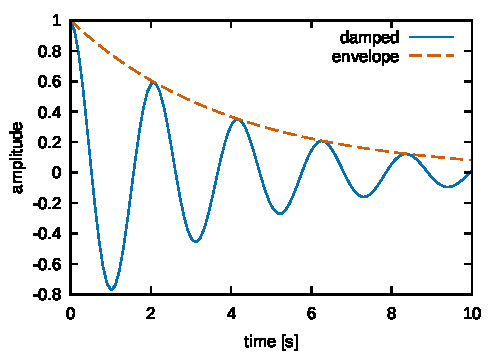
\includegraphics{cb_paper}
  \caption{A column figure: \texttt{theme paper}, 8\,pt texts, 0.75\,pt lines.}
  \label{fig:paper}
\end{figure}

\begin{figure}[t]
  \centering
  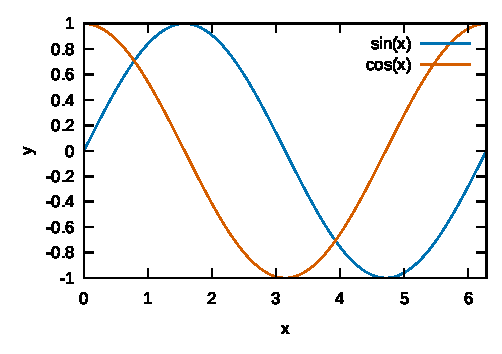
\includegraphics{pc03}
  \caption{The column size, \texttt{size single}: 8.5 by 6\,cm.}
  \label{fig:sizes}
\end{figure}

\section{Frequency response}
The gain $|H(i\omega)| = 1/\sqrt{(1 - \omega^2)^2 + (2 \zeta \omega)^2}$ peaks near the natural frequency for small
damping ratios $\zeta$ (Figures~\ref{fig:double} and~\ref{fig:panels}); the phase turns by half a period across it.

\begin{figure*}[t]
  \centering
  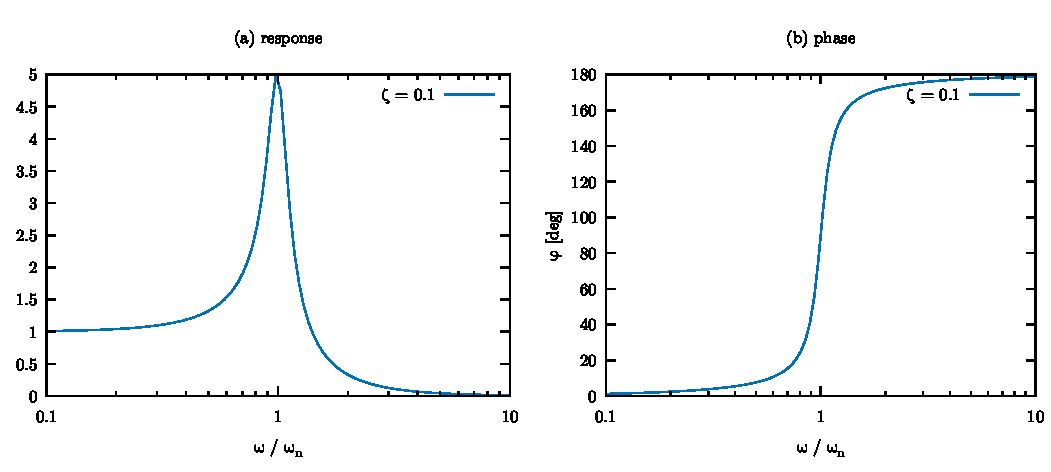
\includegraphics{cb_paper_double}
  \caption{Two panels across the page, in Latin Modern Roman: \texttt{size double theme paper serif}.}
  \label{fig:double}
\end{figure*}

\begin{figure*}[t]
  \centering
  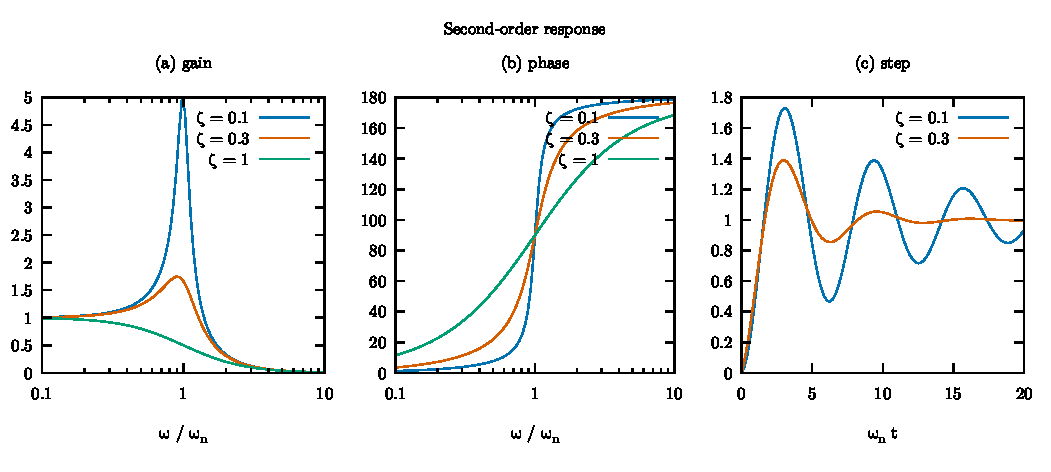
\includegraphics{pc04}
  \caption{Three panels of a multiplot layout under its title.}
  \label{fig:panels}
\end{figure*}

\section{Conclusion}
A figure made for its column needs nothing but \verb|\includegraphics|: no scaling, no converter, its fonts travel
with it.

\end{document}
